\chapter{Inserting Figures and Tables}
\section{Inserting Figures}
\subsection{Inserting Sigle image}

\chapter{EXPERIMENTS}
\vspace{.5cm}
\section{MATERIALS USED}
The materials used for the modified bituminous mix are :
\begin{enumerate}
\item Aggregate
\item Bitumen binder
\item Filler
\item Waste polythylene
\end{enumerate}



\section{MARSHALL TEST}
\vspace{.5cm}
In this method, the resistance to plastic deformation of a compacted cylindrical specimen of bituminous mixture is measured when the specimen is loaded diametrically at a deformation rate of 50 mm per minute. The two major features of the Marshall method of mix are design density-voids analysis and stability-flow tests. The Marshall stability of the mix is defined as the maximum load carried by the specimen at a standard test temperature of 60°C. The flow value is the deformation that the test specimen undergoes during loading upto the maximum load. Flow is measured in 0.25 mm units. In this test, an attempt is made to obtain optimum binder content for the type of aggregate mix used and the expected traffic intensity.

\subsection{Apparatus}
\vspace{.5cm}
\begin{enumerate}
\item Mold Assembly: cylindrical moulds of 10 cm diameter and 7.5 cm height consisting of a base plate and collar extension.
\item Sample Extractor: for extruding the compacted specimen from the mould.
\item Compaction pedestal and hammer.
\item Breaking head.
\item Loading machine.
\item Flow meter , water bath, thermometers.
\end{enumerate}

\subsection{Procedure}
\vspace{.5cm}
In the Marshall test method of mix design three compacted samples are prepared for each binder content. At least four binder contents are to be tested to get the optimum binder content. All the compacted specimens are subject to the following tests:
\begin{itemize}
\item Bulk density determination.
\item Stability and flow test.
\item Density and voids analysis.
\end{itemize}
The coarse aggregate, fine aggregate, and the filler material should be proportioned so as to fulfill the requirements of the relevant standards. The required quantity of the mix is taken so as to produce compacted bituminous mix specimens of thickness 63.5 mm approximately. 1200 gm of aggregates and filler are required to produce the desired thickness. The aggregates are heated to a temperature of 175° to 190°C the compaction mould assembly and rammer are cleaned and kept pre-heated to a temperature of 100°C to 145°C. The bitumen is heated to a temperature of 121°C to 138°C and the required amount of first trial of bitumen is added to the heated aggregate and thoroughly mixed. The mix is placed in a mould and compacted with number of blows specified. The sample is taken out of the mould after few minutes using sample extractor.\\The bulk density of the sample is usually determined by weighting the sample in air and in water. It may be necessary to coat samples with paraffin before determining density. The specific gravity of the specimen is given by
\begin{equation}
\end{equation}.
In conducting the stability test, the specimen is immersed in a bath of water at a temperature of 60° ± 1°C for a period of 30 minutes. It is then placed in the Marshall stability testing machine and loaded at a constant rate of deformation of 5 mm per minute until failure. The total maximum in kN (that causes failure of the specimen) is taken as Marshall Stability. The stability value so obtained is corrected for volume. The total amount of deformation is units of 0.25 mm that occurs at maximum load is recorded as Flow Value. The total time between removing the specimen from the bath and completion of the test should notexceed 30 seconds.

\section{DRAIN DOWN TEST}
In this test,the wire basket method is used. In this test, the laboratory prepared loose mix was taken in the wire basket and is then placed in a forced draft oven for 1 hour at a pre-selected temperature. At the end of 1 hour,the basket containing the sample is removed from the oven along with the plate and the mass of the plate was determined. The amount of increased weight of the plate is the amount of drain down of the mix. The oven temperature for performing the drain down test should be at the mixing temperature or the mixing temperature plus 15 C. Thus, an oven temperature of 175 C was used for the test.

\section{MOISTURE STABILITY TEST}
\vspace{.5cm}
In this test,the water susceptibility of the mix is determined.. The difference in the stability loss of mixtures with and without plastic is determined by immersing the 6 Marshall samples for each plastic content in the water bath at 60 C. The Stability values for three samples from each mixture were obtained after 35 minutes of water immersion and the remaining samples were tested after 24 hours of water immersion.

\section{RUTTING TEST}
\vspace{.5cm}

If you want to add a new figure use the following commands.The file should be saved in the folder named $images$ in order to link the file. Note that the file is centred using $centering$ command, file is linked using $includegraphics$ command. Note how the height and width of the image is specified here. In order to include tour image file here, just replace $manual.png$ with the name of your file. The name of figure should not be having blank spaces. 

\begin{figure}[H]

\centering
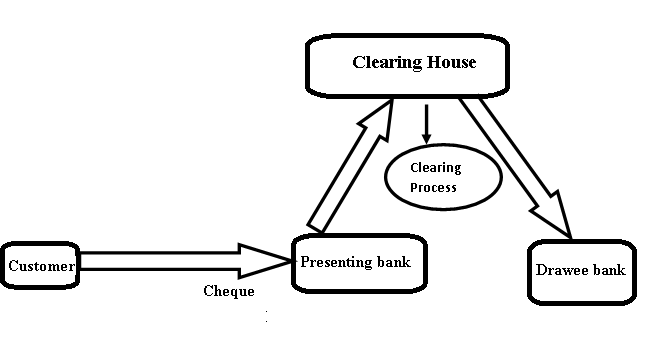
\includegraphics[width=\linewidth,height=5cm] {./images/manual.png}
\caption{Architecture of manual processing of cheques}
\label{manual}
\end{figure}

You might have noticed that the content specified by the command $caption$ is used as the caption of the figure and is automatically numbered. You can see that the figure number, caption of the figure and the page number is automatically generated in list of figures. The keyword $manual$ is set as the label of the figure. The reference to the figure can be inserted in the text by using $ref$ command like this - as shown in Figure \ref{manual}.


\subsection{Inserting more than one images}

Sub figures can be inserted in main figure as shown below. Figure \ref{fig:partitionscheme} shows the output.
\begin{figure}[H]
	
	\centering
	\subfloat[Secret image]
	{
		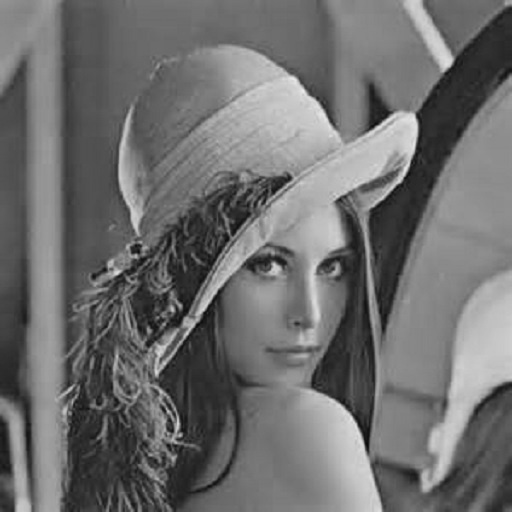
\includegraphics[width=0.25\textwidth]{./images/lena}
		
	}
	\\
	\subfloat[Share1]
	{
		
\includegraphics[width=0.25\textwidth]{./images/lenashare2_1}
		
	}
	\subfloat[Share2]
	{
		
\includegraphics[width=0.25\textwidth]{./images/lenashare2_2}
		
	}
	\subfloat[Share3]
	{
		
\includegraphics[width=0.25\textwidth]{./images/lenashare2_3}
		
	} \\
	\subfloat[Reconstructed image]
	{
		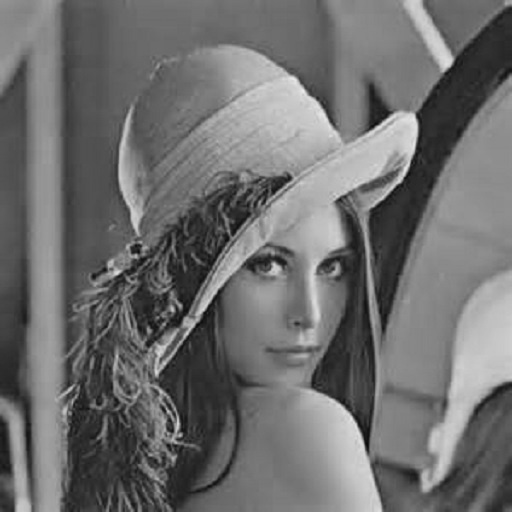
\includegraphics[width=0.25\textwidth]{./images/lena_Original}
		
	}     
	\caption{Result of partition scheme}
	\label{fig:partitionscheme}
\end{figure}

\section{Inserting Tables}
Table are very essential to present information in a report. A basic table is included here as an example. You can change the orrientation to landscape by using the $landscape$ command. The table can be reffered in the text using $ref$ command like - as shown in Table \ref{weather} 

%\begin{landscape}
\begin{table}[H]
\begin{center}
	\caption{\bf Comparison of different schemes}
	\label{weather}
	\begin{tabular}{ | l | l | l | p{5cm} |}
		\hline
		\textbf{Day} & \textbf{Min Temp} & \textbf{Max Temp} & \textbf{Summary} \\ \hline
		Monday & 11C & 22C & A clear day with lots of sunshine.  
		However, the strong breeze will bring down the temperatures. \\ \hline
		Tuesday & 9C & 19C & Cloudy with rain, across many northern regions. Clear spells 
		across most of Scotland and Northern Ireland, 
		but rain reaching the far northwest. \\ \hline
		Wednesday & 10C & 21C & Rain will still linger for the morning. 
		Conditions will improve by early afternoon and continue 
		throughout the evening. \\
		\hline

	\end{tabular}
\end{center}
\end{table}
%\end{landscape}

More information on table can be found at\\ https://en.wikibooks.org/wiki/LaTeX/Tables